\documentclass{standalone}
\usepackage{tikz}
\usetikzlibrary{shapes.geometric, arrows}

\tikzstyle{particleb} = [circle, minimum size=2cm, text centered, fill=red!50]
\tikzstyle{particleg} = [circle, minimum size=2cm, text centered, fill=blue!50]
\tikzstyle{particle1} = [circle, minimum size=2cm, text centered, fill=green!50]
\tikzstyle{particle2} = [circle, minimum size=2cm, text centered, fill=green!25]

\begin{document}

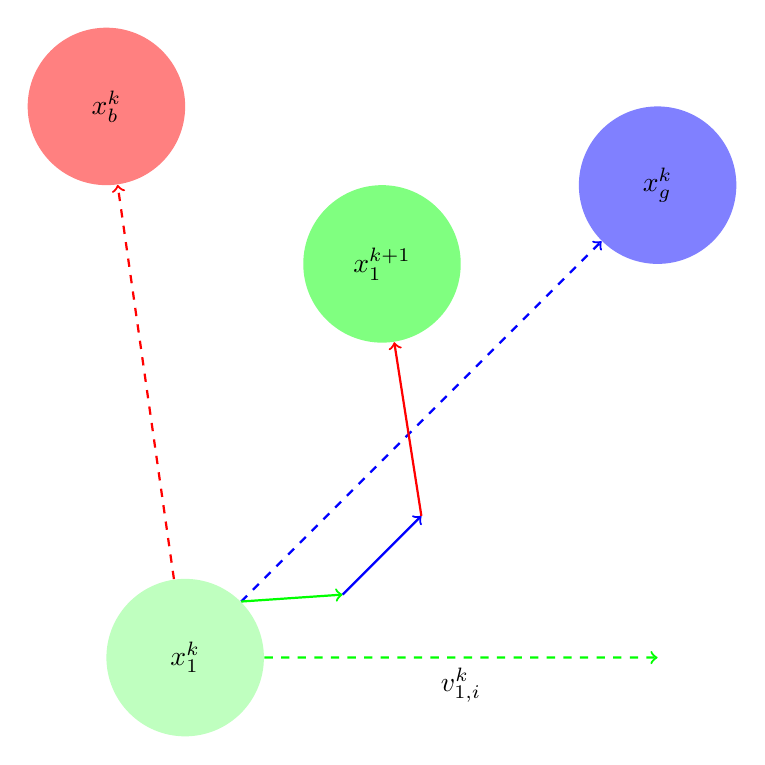
\begin{tikzpicture}[node distance=2cm]

\tikzstyle{particleb} = [circle, minimum size=2cm, text centered, fill=red!50]
\tikzstyle{particleg} = [circle, minimum size=2cm, text centered, fill=blue!50]
\tikzstyle{particle1} = [circle, minimum size=2cm, text centered, fill=green!50]
\tikzstyle{particle2} = [circle, minimum size=2cm, text centered, fill=green!25]


    \node (p1) [particleb] {$x^k_b$};
    \node (p2) [particleg,right of=p1, xshift=5cm,yshift=-1cm] {$x^k_g$};
    \node (p3) [particle1,right of=p1, yshift=-2cm,xshift=1.5cm] {$x^{k+1}_1$};
    \node (p4) [particle2,below of=p1, yshift=-5cm,xshift=1cm] {$x^k_1$};

    \draw [dashed,->,red,thick] (p4) -- (p1);
    \draw [dashed,->,blue,thick] (p4) -- (p2);
    \draw [dashed,->,green,thick] (p4) -- node[anchor=north,black] {$v^k_{1,i}$} (7,-7);
    \draw [->,green,thick] (p4.north east) -- (3,-6.2);
    \draw [->,blue,thick] (3,-6.2) -- (4,-5.2);
    \draw [->,red,thick] (4,-5.2) -- (p3);
\end{tikzpicture}
\end{document}
